\subsection{Komparatorenschaltung} % (fold)
\label{sub:Komparatorenschaltung}
\begin{frame}
\frametitle{Komparatoren}
\framesubtitle{}
    \begin{block}{Komparatoren}
        \begin{figure}[H]
        \begin{center}
                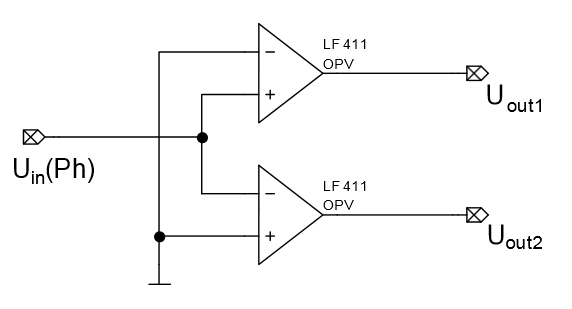
\includegraphics[scale=0.5]{./img/schaltung/Komparatoren.png}
        \end{center}
        \end{figure}
         \begin{itemize}
             \item Wandlung des Sinus-Signals in Rechteckssignal
         \end{itemize}
    \end{block}
\end{frame}

\begin{frame}
\frametitle{Komparatoren}
\framesubtitle{}
    \begin{columns}[c]
        \column{0.6\textwidth}
            \begin{block}{Funktionsweise}
                 \begin{itemize}
                     \item Funktion wie Komparator aus Versuch ??? 
                        \begin{equation*}
                        U_{out}=
                            \begin{cases} 
                                U_{CC} \quad \text{falls} \quad U_1 > U_2 \\
                                U_{EE} \quad \text{falls} \quad U_1 < U_2
                            \end{cases}
                        \end{equation*}
                    \item Sinus and Komparator erzeugt Rechteckssignal
                     \item Anschlüsse entgegengesetzt geschalten $\rightarrow$ Signale
                     gegengleich
                 \end{itemize}
            \end{block}
        \column{0.4\textwidth}
            \begin{figure}[H]
            \begin{center}
                    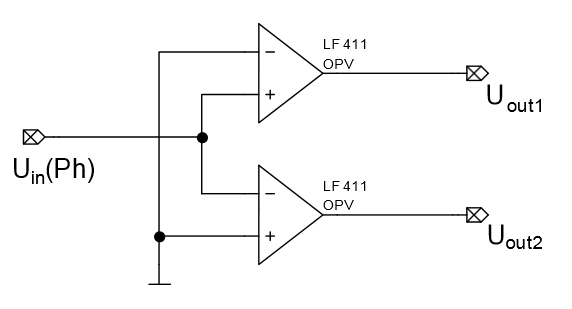
\includegraphics[scale=0.3]{./img/schaltung/Komparatoren.png}
            \end{center}
            \end{figure}
    \end{columns}
\end{frame}

\begin{frame}
\frametitle{Komparatoren}
\framesubtitle{Messungen}
    \begin{columns}[c]
        \column{0.5\textwidth}
             \begin{figure}[H]
             \begin{center}
                     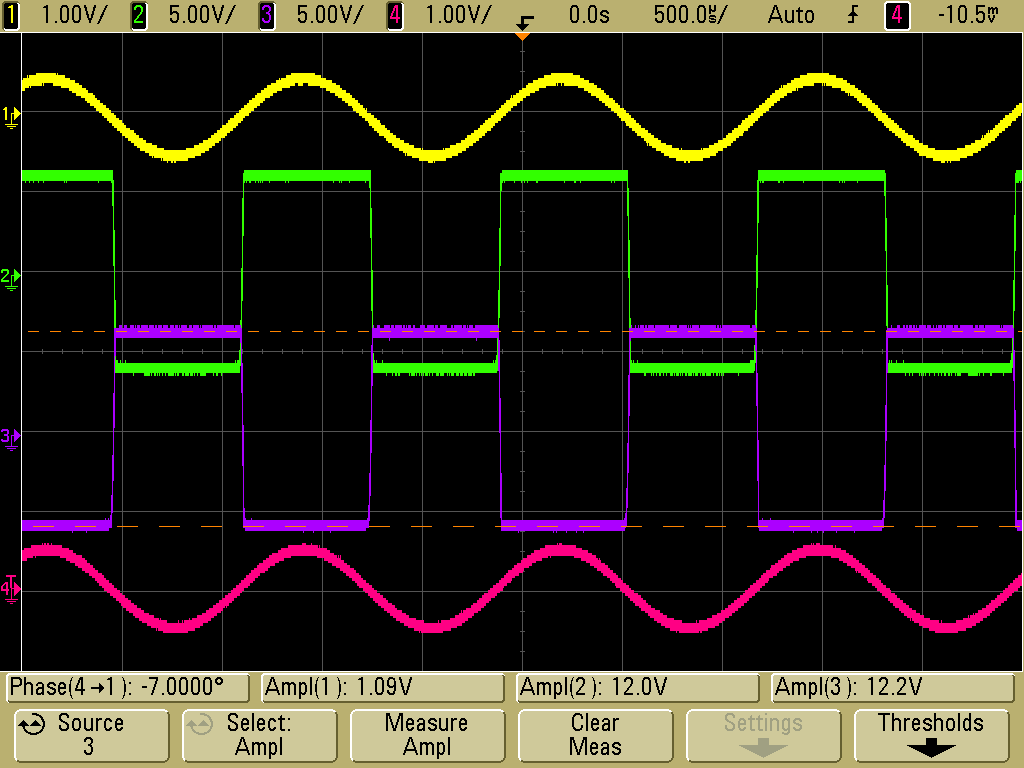
\includegraphics[scale=0.15]{./img/oszi/scope_13.png}
             \end{center}
             \caption{ohne Phasenverschiebung}
             \end{figure}
        \column{0.5\textwidth}
             \begin{figure}[H]
             \begin{center}
                     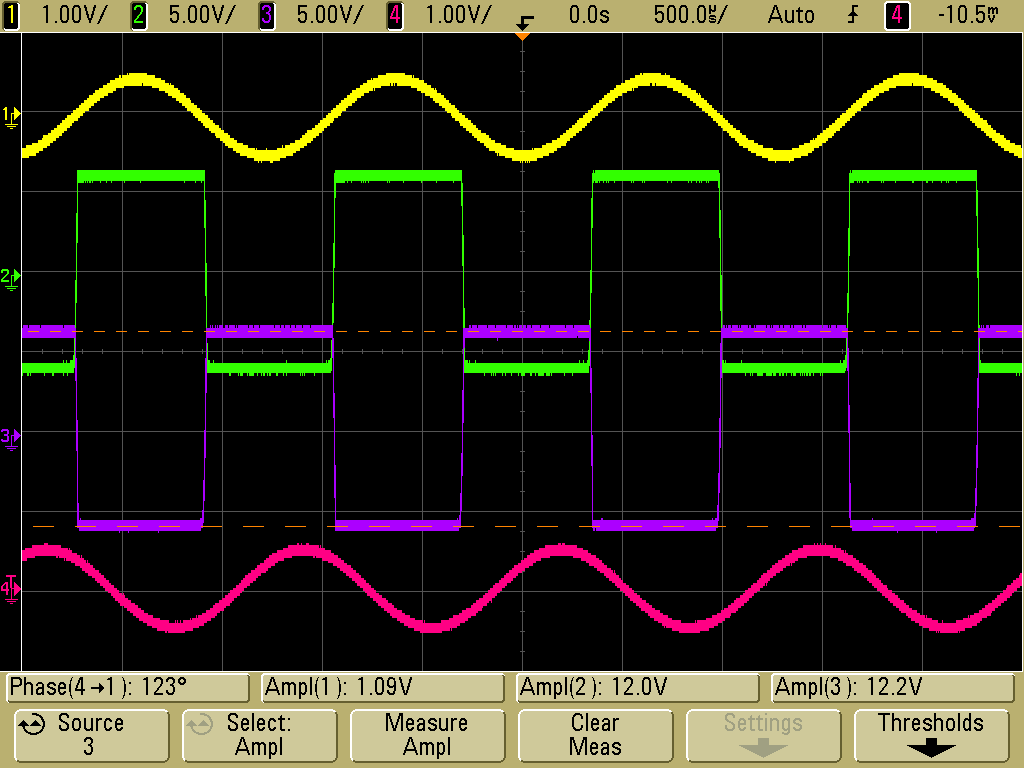
\includegraphics[scale=0.15]{./img/oszi/scope_14.png}
             \end{center}
             \caption{mit Phasenverschiebung}
             \end{figure}
    \end{columns}
    \begin{block}{Bemerkung}
        \begin{itemize}
            \item Amplituden erreichen nicht ganz $14V$
        \end{itemize}
    \end{block}
\end{frame}

% subsection Komparatorenschaltung (end)
